\documentclass[a4paper, 14pt]{extarticle}
\usepackage[a4paper, nohead, left=30mm, right=20mm, top=20mm, bottom=20mm]{geometry}
\usepackage[english, russian]{babel}
\usepackage[T1, T2A]{fontenc}
\usepackage[utf8x]{inputenc}
\usepackage{amsthm}
\usepackage{amssymb}
\usepackage{float}
\usepackage{graphicx}
\usepackage[ruled]{algorithm}
\usepackage{algorithmic}
\usepackage{array}
\usepackage{lscape}
\usepackage{ulem}

\graphicspath{{../figures/eps/bw/}}

%\linespread{1.3}
%\renewcommand{\rmdefault}{ftm}

\def\figureref#1{Рис.\,\protect\ref{#1}}
\def\eqref#1{(\protect\ref{#1}\protect)}

\floatname{algorithm}{Алгоритм}
\theoremstyle{plain}
\newtheorem{theorem}{Теорема}
\newtheorem{lemma}{Лемма}
\theoremstyle{definition}
\newtheorem{definition}{Определение}

\begin{document}
	\Russian

	\begin{titlepage}
{
	\newpage
	\fontsize{14pt}{22pt}

	\begin{center}
	{
		\fontsize{12pt}{20pt} \sf
		\mbox{ УЧРЕЖДЕНИЕ РОССИЙСКОЙ АКАДЕМИИ НАУК }\\[5pt]
		\mbox{ САНКТ-ПЕТЕРБУРГСКИЙ АКАДЕМИЧЕСКИЙ УНИВЕРСИТЕТ –- НАУЧНО- }\\
		\mbox{ ОБРАЗОВАТЕЛЬНЫЙ ЦЕНТР НАНОТЕХНОЛОГИЙ РАН }
	}
	\end{center}

	\vspace{20pt}
	\hfill
	\begin{minipage}{220pt}
		\begin{center}
		{
			\fontsize{12pt}{20pt}
			На правах рукописи\\[15pt]
			Диссертация допущена к защите\\
			Зав. кафедрой\\
			\vspace{10pt}
			\hspace{10pt}\hrulefill\hspace{10pt} \\
			\vspace{5pt}
			\hspace{25pt} ``\hspace{20pt}'' \hrulefill\hspace{5pt}2010 г. \hspace{25pt}
		}
		\end{center}
	\end{minipage}

	\vspace{30pt}
	\begin{center}
	{
		{ \bf ДИССЕРТАЦИЯ } \\
		{ НА СОИСКАНИЕ УЧЕНОЙ СТЕПЕНИ } \\[5pt]
		{ \bf МАГИСТРА } \\
	}
	\end{center}

	\vspace{10pt}
	\begin{flushleft}
	{
		Тема: Алгоритмическое перечисление альтернированных $k$-танглов \\
		\vspace{10pt}
		Направление: 010600.68 –- Прикладные математика и физика \\
		\vspace{10pt}
		Магистерская программа: ``Математические и информационные технологии'' \\
	}
	\end{flushleft}

	\vspace{20pt}
	\begin{flushleft}
		{ Выполнил студент \hfill А. С. Мишунин} \\
		\begin{center} { \fontsize{8pt}{0pt} (подпись) } \end{center}
		{ Руководитель:\\д. ф. - м. н., профессор \hfill А. В. Омельченко} \\
		\begin{center} { \fontsize{8pt}{0pt} (подпись) } \end{center}
		{ Рецензент:\\к. ф. - м. н., доцент \hfill В. Р. Мешков}
		\begin{center} { \fontsize{8pt}{0pt} (подпись) } \end{center}
	\end{flushleft}

	\vfill
	\begin{center}
	{
		Санкт-Петербург \\[5pt]
		2010 г.
	}
	\end{center}
}
\end{titlepage}

	\setcounter{page}{2}

	\newpage
\renewcommand{\abstractname}{Реферат}
\begin{abstract}
	Данная работа состоит из введения, трех глав основной части, заключения и списка литературы. Написана на 30 листах.
	Содержит 23 иллюстрации, 4 таблицы и 3 листинга алгоритма. Список литературы содержит 19 наименований.

	Результатом работы является описание алгоритма, который позволяет генерировать все возможные простые связные
	альтернированные $k$-танглы с количеством перекрестков, не превосходящим заданное число. Основными его достоинствами
	по сравнению с аналогичными для узлов и зацеплений являются отсутствие необходимости в больших хеш-таблицах, малый по
	сравнению с общим количеством генерируемых объектов объем необходимой памяти со случайным доступом и малый объем
	выполняемой заведомо бесполезной работы.
	
	Также в работе описан алгоритм рисования диаграмм $k$-танглов.

	%\listoffigures
	%\listoftables
	%\listofalgorithms
\end{abstract}


	\newpage
	\renewcommand{\contentsname}{Оглавление}
	\tableofcontents

	\newpage
\section{Введение}

	\subsection{Некоторые определения}

	\begin{figure}[ht]
		\centering
		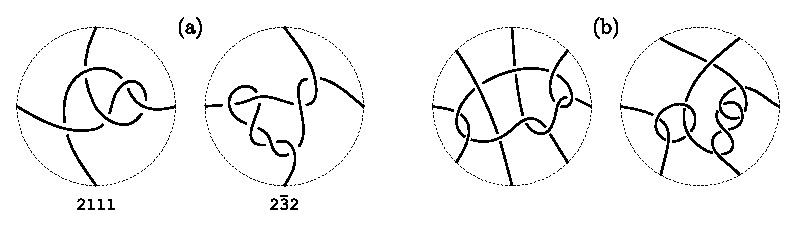
\includegraphics{c/tangles-example.eps}
		\caption{$2$-танглы (a), $k$-танглы в общем случае (b)\label{figure:tangles-example}}
	\end{figure}

	\begin{definition}
		\label{definition:tangle}
		$k$-танглом называется гладкое вложение $k$ отрезков и конечного числа окружностей в $B^3$
		(трехмерный замкнутый шар единичного радиуса), если $2k$ концов отрезков взаимно однозначно отображаются
		на точки с координатами $(\cos\pi i/k, \sin\pi i/k, 0)$, $i\in\{0, 1, \dots, 2k{-}1\}$, называемые
		концами $k$-тангла, и больше ни какие точки отрезков или окружностей на границу $B^3$ не отображаются.
	\end{definition}

	\begin{definition}
		\label{definition:tangle-equiv}
		$k$-танглы $T_1$ и $T_2$ называются эквивалентными, если существует изотопия $B^3$, сохраняющая границу
		неподвижной, которая переводит $T_1$ в $T_2$.
	\end{definition}

	\begin{definition}
		$k$-танглы $T_1$ и $T_2$ называются слабо эквивалентными, если существует изотопия $B^3$ (не обязательно
		сохраняющая границу неподвижной) которая переводит $T_1$ в $T_2$.
	\end{definition}

	\begin{figure}[ht]
		\centering
		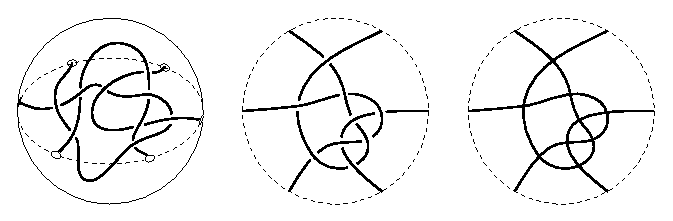
\includegraphics{c/tangle-diagram-projection.eps}
		\caption{$3$-тангл, его диаграмма и проекция\label{figure:3-tangle-and-proj}}
	\end{figure}

	Аналогично узлам и зацеплениям мы можем ввести понятие диаграммы и для $k$-танглов, строя невырожденные проекции
	$k$-тангла на плоскость, проходящую через его концы. Из \figureref{figure:tangles-example} \figureref{figure:3-tangle-and-proj}
	можно получить интуитивное представление о том, что такое диаграммы; строгое определение и подробное обсуждение
	``тонких мест'', напрямую не относящихся к нашей текущей теме, читатель может найти, например, в книге \cite{Cromwell2004}.
	Диаграммы, которые отличаются только плоской изотопией, сохраняющей граничную окружность, мы различать не будем.

	\begin{definition}
		Перекрестками диаграммы (проекции) называются точки, в которые проецируются две точки $k$-тангла. Ребрами
		диаграммы (проекции) называются максимальные множества точек, не лежащие на границе, в которые проецируется
		только по одной точке $k$-тангла.
	\end{definition}

	Ребра гомеоморфны открытым отрезкам и соединяют либо 2 перекрестка, либо 2 конца $k$-тангла либо конец с перекрестком.

	\begin{definition}
		Минимальной диаграммой $k$-тангла $T$ называют диаграмму $T$ с минимальным количеством перекрестков.
	\end{definition}

	\begin{figure}[ht]
		\centering
		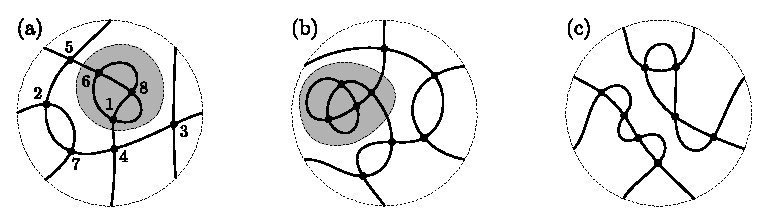
\includegraphics{c/composite-non-connected-projections.eps}
		\caption{Составные (a, b) и несвязные (c) проекции\label{figure:composite-proj}}
	\end{figure}

	\begin{definition}
		Диаграмма (проекция) $k$-тангла называется составной, если строго внутри граничной окружности существует замкнутая
		гладкая несамопересекающаяся кривая, которая трансверсально пересекает диаграмму ровно в двух точках и содержит
		внутри как минимум один перекресток. В противном случае диаграмма называется простой.
	\end{definition}

	\begin{definition}
		$k$-тангл называется простым, если просты все его минимальные диаграммы.
	\end{definition}

	\begin{definition}
		Диаграмма (проекция) называется связной, если граф, ребрами которого являются ребра диаграммы (проекции), а
		вершинами --- вершины и концы диаграммы (проекции), является связным.
	\end{definition}

	\begin{definition}
		$k$-тангл называется связным, если связна любая его диаграмма.
	\end{definition}

	\begin{definition}
		Диаграмма $k$-тангла называется альтернированной, если у каждого ребра, соединяющего два перекрестка, один из
		концов проходит над перекрестком, а другой --- под.
	\end{definition}

	\begin{definition}
		$k$-тангл называется альтернированным, если он имеет альтернированную диаграмму.
	\end{definition}


	\subsection{Постановка задачи}

	Как и в случае с узлами и зацеплениями, было бы логично поставить задачу классификации и для $k$-танглов. На настоящий
	момент результаты в этой области имеются в основном только для $2$-танглов. Общий случай уже интересен сам по себе,
	более того $k$-танглы могут оказаться полезными для исследованиях в других областях, например, для представления узлов
	и зацеплений в замкнутых ориентируемых поверхностях произвольного рода \cite{Kauffman1999, Kuperberg2003} --- так называемых
	виртуальных узлов и зацеплений.

	Так в работе \cite{Conway1970} J.~Conway ввел понятие танглов (которые в соответствии с Определением~\ref{definition:tangle}
	являются $2$-танглами) в качестве средства для описания и классификации узлов и зацеплений. Там же была предложено разделение
	танглов на классы рациональных, алгебраических и трансцендентных. Самым поддающимися исследованию оказались рациональные
	танглы --- для них проблема классификации была полностью решена \cite{KauffmanLambropoulou2004}.

	Для простых альтернированных $2$-танглов было получено полиномиальное уравнение на производящую функцию
	\cite{SundbergThistlethwaite1998}, которое затем было использовано там же для улучшения оценок на количество простых
	альтернированных зацеплений.

	Матричные интегралы рассматриваются как средство для перечисления альтернированных $k$-танглов в
	\cite{Justin1999_1, Justin1999_2, JustinZuber2000, Justin2001, JacobsenJustin2002, JustinZuber2003}.
	Там приведены теоретические результаты,	а также численно полученная таблица количеств простых альтернированных 
	$2$- и $3$-танглов. Однако сложность предложенного метода быстро растет с увеличением $k$.

	Наконец в \cite{KanenobuSaitoSatoh2003} с точностью до слабой эквивалентности были классифицированы простые $2$-танглы
	не более, чем с семью перекрестками.

	Целью данной работы является алгоритм, позволяющий получить все альтернированные $k$-танглы (а точнее их минимальные диаграммы)
	с количеством перекрестков, не превосходящим заданное число. Иными словами проделать то же самое для альтернированных танглов,
	что было сделано в \cite{Rankin2002_1, Rankin2002_2, Rankin2002_3} для альтернированных зацеплений. Однако, класс рассматриваемых
	$k$-танглов стоит ограничить уже по той причине, что всего их, даже с конечным числом перекрестков, бесконечное число. Поэтому
	мы будем рассматривать только связные альтернированные танглы. Также из рассмотрения традиционно исключаются составные
	диаграммы --- так мы и будем поступать.

	Выбор класса альтернированных $k$-танглов обусловлен рядом их известных свойств, сильно облегчающих задачу. В частности,
	любая минимальная диаграмма простого альтернированного тангла является альтернированной и, кроме того, все его минимальные диаграммы
	могут быть получены друг из друга применением (возможно, многократным) преобразования, называемого ``flype''
	(см. \figureref{figure:flype}). Также любая нередуцируемая (т. е. такая, в которой нельзя сразу же ``распутать'' петлю
	первым движением Редемейстера, тем самым уменьшив число перекрестков), в частности --- простая, альтернированная диаграмма
	является минимальной диаграммой.

	\begin{figure}[ht]
		\centering
		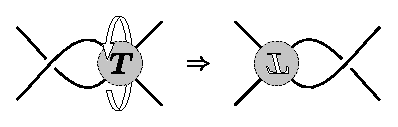
\includegraphics{c/flype.eps}
		\caption{Flype\label{figure:flype}}
	\end{figure}

	P.~G.~Tait более 100 лет назад \cite{Tait1900} выдвинул предположение о возможности получения минимальных альтернированных диаграмм
	узлов и зацеплений друг из друга с помошью преобразования \figureref{figure:flype}, получившее название ``Tait flyping conjecture''.
	Доказано оно было относительно недавно W.~Menasco и M.~Thistlethwaite в \cite{MenascoThistlethwaite1991, MenascoThistlethwaite1993},
	а утверждения выдвинутые выше являются являются его простыми обобщениями и следствиями.

	Как правило в литературе (в нашем случае это во всех ссылках, кроме \cite{KanenobuSaitoSatoh2003}) для перечисления танглов
	используются аналитические методы, поэтому там используется Определение~\ref{definition:tangle-equiv} для определения эквивалентности
	двух $k$-танглов, так как оно дает наиболее простые соотношения. Мы, однако, собираемся явно получать проекции всех простых связных
	альтернированных $k$-танглов с количеством перекрестков не превосходящим заданное число, значит заинтерисованы в максимальном сокращении
	количества ненужной работы. Поэтому имеет смысл отождествлять две диаграммы $k$-танглов, отличающиеся действием элемента
	группы $D_{2k}$ в дополнение к разрешенным Определением~\ref{definition:tangle-equiv} преобразованием. Очевидно, что большая часть
	танглов несимметрична, поэтому уже для $2$-танглов мы получаем выигрыш почти в 8 раз, а с ростом $k$ он становится все более
	значительным.

	Схема дальнейшей части работы выглядит следующим образом: в Главе~\ref{section:projections} мы рассмотрим алгоритм генерации
	всех возможных неэквивалентных (с точностью до плоской изотопии и $D_{2k}$) простых связных проекций $k$-танглов, затем мы
	покажем как модифицировать его для генерации простых альтернированных танглов в Главе~\ref{section:alternating}. Наконец,
	в Главе~\ref{section:drawing} приводится алгоритм создания ``красивых'' изображений $k$-танглов, который, конечно,
	непосредственного отношения к рассматриваемым вопросам не имеет, но является настолько полезным в процессе исследования, что
	фактически без него невозможно обойтись.

	\documentclass[12pt]{article}
%\usepackage[cp1251]{inputenc}
%\usepackage[english,russian]{babel}
\usepackage[a4paper,nohead,left=20mm,right=20mm,top=20mm,bottom=20mm]{geometry}
\usepackage{local}

\parindent=0mm
\parskip=3mm

\begin{document}

\title{Classification of $k$-tangle projections using cascade representation}

\author{A. Bogdanov, V. Meshkov, A. Omelchenko, M. Petrov\\
St Petersburg Polytechnic University, St Petersburg, Russia}

\abstract{The paper addresses the $k$-tangle enumeration problem. We introduce a notion of
cascade diagram for $k$-tangle projections. An effective enumeration algorithm for projections is
proposed based on cascade representation. Tangles projections with up to 12 crossings are
tabulated. We provide also pictures of alternating $k$-tangles with 5 crossing or less.}

\maketitle

\section*{Introduction}

Tangles (see~\picref{conway.eps}) were introduced by John Conway \cite{Conway1970} as an
instrument for the description and classification of knots and links. According to up-to-date
definitions~\cite{Cromwell2004}, Conway's tangles are 2-tangles. A natural generalization of
2-tangles are $k$-tangles or $k$-string tangles (\picref{conway.eps}b), where $k$ is one-half of
the number of ``legs''.

As in the case of knots and links we can consider the classification problem for %the class of
$k$-tangles. This problem is only solved for some specific subclasses of
2-tangles~\cite{Kanenobu2003,Kauffman2004} (e.\,g.~rational tangles) which are most-used for
studying knots. The general case of $k$-tangles is interesting in itself. Furthermore it is
possible to use $k$-tangles for representing knots and links in a ``thickened'' closed oriented
surface of arbitrary genus (virtual links~\cite{Kauffman1999,Kuperberg2003}). So $k$-tangle
classification can be a basis for classifying virtual links.

% In special case $g=1$ such knots describe ``textile'' structures (double periodic links)~\cite{We2005}.

\centerpic{conway.eps}{2-tangles (Conway's notation) (a), $k$-tangles in general case (b)}

In this paper we introduce a notion of cascade diagram and propose a classification algorithm for
$k$-tangles based on the cascade representation. We represent cascade diagrams by a code that is
almost as compact as DT-code (Dowker--Thistlethwaite) for knots \cite{Dowker1983}. This cascade
code actually is a recipe for how to draw the projection, so there is no problem with
verification of realizability of a given code.

The first step in most knots enumeration algorithms is enumeration of projections. Having the
full set of projections with $n$ crossings, it is easy to generate all the knots (links, tangles)
by arranging under- and over-crossing in each projection by all $2^n$ possible ways
\cite{Hoste2006}.

Projection enumeration is related directly to enumeration of alternating knots (links, tangles).
For any projection it is possible to arrange crossings in such a way that ``under'' and ``over''
will alternate when traveling along each component of the link (tangle). It is known that a
(reduced) alternating diagram of a given link has minimal number of crossings (Tait conjecture).
Any projection determines uniquely (up to mirror symmetry) an alternating knot (link, tangle).
However, the set of projections with $n$ crossings is wider than the set of alternating
knots (links, tangles): %according to famous Tait flipping conjecture proved by Menasco and Thistlewaite,
all alternating diagrams obtained from a given one by a series of flype (\picref{flyp.eps})
correspond to the same knot (link, tangle).

\centerpic{flyp.eps}{A flype}

In this paper we will concentrate first of all on the classification of tangle projections.

%In the paper the coding procedure of $k$-tangle projections is offered on the base of its
%representation as cascade diagrams. The enumeration algorithm of $k$-tangle projections with
%fixed number $n$ of crossings is described accurate within the reflections in a plane and the
%rotations.


\section{Basic definitions}\label{defs}

\begin{dfn} A proper embedding of a disjoint union of $k$ arcs and (possibly) some
number of circles into the standard $3$-ball $B^3$ is called a {\it $k$-tangle.} The $2k$
endpoints are fixed at the points $(\cos\pi i/k,\sin\pi i/k,0)$, $i\in\{0,1,\dots,2k{-}1\}$ on
the boundary sphere~(\picref{ball.eps}). $k$-tangle is considered up to the dihedral symmetry
group $D_{2k}$.\end{dfn}

\begin{dfn} Tangles $T_1$ and $T_2$ are {\it equivalent\/} if there is an isotopy i.\,e.~a
smooth family $f_t\,{:}\;B^3\to B^3$, $t\in[0,1]$ of smooth homeomorphisms on the ball that keep
the boundary sphere fixed such that $f_0=\mathrm{id}$ and tangles $T_2$ and $\tilde T_1=f_1(T_1)$
are congruent up to dihedral group transformations.\end{dfn}

\centerpic{ball.eps}{A $3$-tangle, its diagram and projection}

Along with the equivalence defined above a weaker equivalence relation is also considered that
allows the legs of the tangle to be moving on the boundary sphere~\cite{Sundberg1998}.

\begin{dfn}\label{weakeq} Tangles $T_1$ and $T_2$ are {\it weakly equivalent\/} if there is a smooth
family $f_t\,{:}\;B^3\to B^3$, $t\in[0,1]$ of smooth homeomorphisms on the ball $B^3$ such that
$f_0=\mathrm{id}$ and $f_1(T_1)=T_2$.\end{dfn}

In \cite{Kanenobu2003} 2-tangles with 7 crossings or less are classified up to weak equivalence.

For graphical representation of tangles conventional {\it diagrams\/} are used which are
non-singular projections onto the equatorial disk $x^2+y^2\le1$, $z=0$ with additional
information at each double point about which ``thread'' is above the other one
(\picref{ball.eps}b). We are more interested here in projections in themselves
(\picref{ball.eps}c).

\begin{dfn} A tangle projection (diagram) is called {\it composite,} if there is a smooth
closed curve inside the boundary circle that intersects the projection exactly twice and encloses
at least one crossing (\picref{nugatory.eps}a,b). Otherwise the projection is called {\it
prime.}\end{dfn}

\centerpic{nugatory.eps}{Composite (a,b) and non-connected (c) projections}

As in the case of knots and links we are interested in classification of prime projections only.
Moreover, it is natural to consider only connected projections, i.\,e.~such that it is possible
to get from any crossing to any other moving along the arcs of the projection. An example of
non-connected projection is shown in~\picref{nugatory.eps}c.

We will use the terminology of graph theory for description of projections. In particular, the
double points of a projection will be called {\it vertices,} and arcs will be called {\it edges.}
The set of vertices will be denoted by $V$, and the set of edges will be denoted by $E$.

Finally, for the following we need two more definitions.

\begin{dfn} A crossing (vertex) is called a {\it boundary crossing (respectively, vertex)} if some of the
incident edges are connected with the boundary circle.\end{dfn}

\begin{dfn}\label{cut} A {\it cut-crossing (vertex)} is a crossing (vertex) that if removed (together
with the incident edges) produces a non-connected graph.\end{dfn}

For example, the projection \picref{nugatory.eps}a contains five boundary crossings
2,\,3,\,4,\,5,\,7. The crossing number 4 is a cut-crossing.


\section{Cascade diagram of projection}\label{cascade}

Any prime connected projection can be represented as a {\it cascade diagram\/} which is defined
in the following way. Let us construct a system of nested disks in the disk so that there is
exactly one vertex in each annular layer (\picref{cascade.eps}), and a connected sub-projection
is contained inside each area. Of course, this can always be done in many ways.

\centerpic{cascade.eps}{Cascade diagram construction}

Let us cut the disk from the central vertex (vertex~1 in \picref{cascade.eps}) to the boundary
circle so that the cutting line intersects the boundary of each area exactly once (wide-dashed
lines in \picref{cascade.eps}). We allow the cut to dissect the projection at vertices only
(see~\picref{cascade.eps}b). Opening the cut, we obtain a representation of the projection as a
falling cascade (\picref{cascade.eps}). We will call this representation a {\it cascade diagram}
of the projection.

There is only one vertex at each level of the cascade diagram. Edges incident to this vertex
intersect upper and/or lower boundaries of the level. Only five configurations are possible, that
correspond to the patterns
$$
\OI,\ \O,\ \PI,\ \P,\ \X.
$$
The \OI pattern, which is always the starting pattern, cannot be located at lower levels because
of connectivity of the projection and by construction. Moreover, let us prove the following
statement:

\begin{thm}\label{thm1}
Any prime projection has a cascade diagram free of the \O pattern; any vertex can be chosen as
the starting vertex of such a cascade diagram.\end{thm}

We shall prove the theorem by constructing an explicit recurrent algorithm that allows us to
construct the required cascade diagram.

\begin{lmm} Any prime projection has at least two non-cut boundary crossings.\end{lmm}

\centerpic{lemma.eps}{On the proof of the Lemma}

\begin{proof}
Through each cut-crossing draw a chord (a simple curve with end points on the boundary circle)
that nowhere else intersects the projection (\picref{lemma.eps}). It is always possible by
Definition\,\ref{cut}, and can be done in such a way that the chords do not cross each other.
Obviously, there are at least two ``outermost'' chords (e.\,g.~the chords passing through the
crossings 3,\,8,\,9 in \picref{lemma.eps}). Any of these chords cuts a ``lune'' (a part of the
disk not containing cut-crossings). But by the cut-crossing definition any lune should contain at
least one crossing; moreover, there is at least one boundary crossing in each lune (the contrary
is possible only for composite projections of type~\picref{nugatory.eps}b). So, for each lune
there is at least one non-cut boundary crossing. This completes the proof.\end{proof}

\begin{proof}[Proof of the Theorem~\ref{thm1}]
Set an arbitrary crossing to be the starting crossing of the cascade. We will build the cascade
diagram in bottom-up direction. Choose one of non-cut boundary crossings that is not the starting
one (this is always possible by the Lemma). Put this crossing on the lower $n$-th level
(see~\picref{cascade.eps}). The residual part of the projection is again a connected prime
projection; it has $n{-}1$ crossings. By the Lemma this projection has at least two non-cut
boundary crossings. So again we can choose a crossing different from the starting one and put it
on the $(n{-}1)$-th level. Repeating this procedure until all the crossings (except the starting
one) will arrange we construct the required cascade diagram.\end{proof}

Thus, any projection can be represented by a cascade diagram containing (besides the starting
pattern \OI) the patterns \PI, \P, \X only; it is easily shown that each of these patterns is
necessary.


\section{Cascade code}

Let us code levels of a cascade diagram starting from the top. The pattern \OI is always on the
first level so we will not include it in the code. For other levels we will use the following
coding scheme. Associate a pair $(\alpha_i,m_i)$ with the $i$-th level of the cascade diagram. We
suppose $\alpha_i$ equals to $-1$, $0$, and $1$ for the patterns $\P$, $\X$, and $\PI$
respectively; an integer $m_i$ determines the shift of the pattern $\alpha_i$ with respect to the
pattern $\alpha_{i-1}$ on the previous level. We choose a reference point for each pattern to
determine the shift $m_i$: the origin on the left leg for the $\X$ pattern, and on the central
leg for the patterns $\P$ and $\PI$. The shift $m_i\in0,1,\dots,k_{i-1}{-}1$ counts in
counterclockwise direction (in left-right direction on cascade diagram).

So a diagram with $n$ crossings is coded by an ordered set of $n{-}1$ pairs:
$$
C=\bigl\{(\alpha_2,m_2),\dots,(\alpha_n,m_n)\bigr\}
$$
(recall that the code does not include the starting pattern $\OI$; also we can always assume that
$m_2$ is zero). For example, the code
$$
C=\bigl\{(1,0),(0,5),(0,3),(0,3),(0,5)\bigr\}
$$
corresponds to the cascade diagram \picref{cascade.eps}b; i.\,e.~the patterns are $\PI$, $\X$,
$\X$, $\X$, $\X$, the (cyclic) shift of the $\X$ at the 3-th level with respect to the preceding
$\PI$ is 5, the shift of the $\X$ at the 4-th level with respect to the previous is 3, and so on.

Cascade code for $k$-tangles with $n$ crossings is almost as compact as the DT-code for knots
with $n$ crossings~\cite{Dowker1983,Rankin2002_1}: we need only 2 bits per crossing additionally
for storing $\alpha_i$. Note that the length of cascade code only depends on the crossing number;
it does not depend on the number of tangle components (and therefore on the number of legs).

Cascade code is actually a recipe for how to draw the projection, so we have no problem with
nonrealizable codes, a nontrivial problem with DT codes. The last property allows us to use the
cascade code effectively for generation and enumeration of tangle projections with a given number
of crossings.

Each projection has a lot of cascade representations so the equivalence problem for cascade codes
occurs. In order to resolve this problem it is necessary to define a {\it canonical cascade
code\/} which should correspond uniquely to a given projection. Such code can be constructed in
different ways. We will define it in such a way that the important {\it nesting property\/} will
be satisfied.
\begin{equation}\label{nesting}\raise-\baselineskip\hbox{\vbox{\hsize=0.75\textwidth \it\noindent
If $C_n=\bigl\{(\alpha_2,m_2),\dots,(\alpha_n,m_n)\bigr\}$ is a canonical cascade code, then any
initial segment $C_i=\bigl\{(\alpha_2,m_2),\dots,(\alpha_i,m_i)\bigr\}$, $2\le i\le n{-}1$, of the
code is again the canonical cascade code of the corresponding sub-tangle with $i$~crossings.}}
\tag{$*$}
\end{equation}
In order to define the canonical cascade code, we will at first define an auxiliary invariant
code of a projection.


\section{Invariant root-code of projection}

\begin{dfn} A {\it root\/} of a projection is a triple $r=(v,e,f)$ where $v\in V$ is a
vertex of the projection, $e\in E$ is one of four edges incident to $v$, $f$ is one of two faces
incident to $e$ (see examples in~\picref{rootnum.eps}). The parts $v$, $e$, and $f$ are called
the {\it root-vertex,} {\it root-edge,} and {\it root-face\/} respectively.\end{dfn}

The location of the root-face relative to the root-edge and the root-vertex determines naturally
a rotation direction (clockwise or counter-clockwise) about the root-vertex which we will call
the {\it labeling direction.}

Vertices of the projection can be uniquely labeled for a fixed root. For example, the following
algorithm may be used:
\begin{quote}\parskip=0mm\ttfamily\footnotesize

0.~~set the number of the root-vertex as 1;

~~~~~~number vertices adjacent to the root-vertex

~~~~~~in the labeling direction starting from the root-edge;

1.~~among the labeled vertices find the vertex $q$

~~~~~~with the smallest number that has unlabeled neighbors;

2.~~assign the numbers to unlabeled vertices around the vertex $q$

~~~~~~in order determined by the labeling direction,

~~~~~~starting from the first unlabeled edge;

3.~~if there are still unlabeled vertices return to the step 1.
\end{quote}

\noindent The vertices of the projection in \picref{rootnum.eps}a,b are labeled using the
algorithm described above.

\centerpic{rootnum.eps}{Two vertex labelings induced by different roots, the adjacency lists;\\
the canonical labeling (b)}

During the labeling algorithm execution an \emph{adjacency list\/} $A_r$ is constructed. The
$i$-th line of the adjacency list contains labels of the vertices adjacent to the $i$-th vertex
listed in the labeling direction. For the boundary vertices we substitute $\mathtt{0}$ at the
positions corresponded to the boundary edges (see~\picref{rootnum.eps}).

The order of numbers in each line of the list is determined up to a cyclic shift. Let us chose
the lexicographically minimal sequence from the four possible variants. (The line
$a=[a_1,\dots,a_n]$ is {\it lexicographically less\/} than line $b=[b_1,\dots,b_n]$ if there is
$j$ such that $a_j<b_j$ and $a_i=b_i$ for any $i<j$.)

Let us agree to write the adjacency list $A_r$ in one line. For example, the root in
\picref{rootnum.eps}a determines the adjacency list
$$
A_r=[\mathtt{0~2~2~3~1~1~4~4~1~5~6~6~0~5~2~2~0~0~3~4~0~0~3~3}].
$$

\begin{dfn} A single-line adjacency list $A_r$ constructed as described above is called the {\it root-code\/}
cor\-re\-spon\-ding to a given root~$r$.\end{dfn}

Thus for a fixed root the corresponding root-code is defined uniquely; in turn a root-code
determines uniquely the corresponding projection (up to rotations and reflections).

We can define a root of a given projection in $8n$ ways. Therefore, there are $8n$ generally
different root-codes of the projection; so in order to define an invariant code we need a rule
that allows us to choose a unique root-code from this set. The root-code constructed by that rule
we will call the {\it canonical} and will denote as $\rcode(\cdot)$.

\begin{dfn} Root-code $\rcode(\cdot)$ is called an {\it invariant root-code\/} if it is
determined uniquely by a given projection:
$$
\rcode(P_1)=\rcode(P_2)\ \Longleftarrow\ P_1\cong P_2.
$$\end{dfn}

For example one of the simplest rules (but in the same time one of the most inefficient) is the
following one: define the invariant root-code as the lexicographic minimum among all $8n$ codes.

In order to construct a canonical cascade code satisfying the nesting property \eqref{nesting} we
need the root-vertex to be {\it boundary\/} and {\it non-cut.} It is obvious that a root-code
will be lexicographically minimal only if the root-vertex has {\it maximum number of legs:} in
this case there will be maximum number of starting zeroes in the root-code. For the projection in
\picref{rootnum.eps}a even these two requirements reduce the search set to two root-vertices 2
and 6.

We can reduce the number of compared codes some more, for example using a face-code notion. Let
us associate an integer with each boundary face --- the number of projection edges adjacent to
the face. Then we can write these numbers for all boundary faces in order defined by the labeling
direction as a string of length~$2k$ (number of legs). The {\it face-code\/} corresponding to a
given (boundary) root is such a sequence that the starting number corresponds to the root-face.
For example the face-code for the root in \picref{rootnum.eps}b is $[\mathtt{2~3~4~4~2~4}]$.

Thus, we select an invariant subset in the set of roots
\begin{equation}\label{rset}
R=\Biggl\{r\;\Biggr|\ \raise-1\baselineskip\vbox{\hsize=17em\noindent
root-vertex is a boundary vertex,\\
root-vertex is a non-cutting vertex,\\
face-code is lexicographically minimal}\Biggr\}.
\end{equation}

Now let us define {\it invariant root-code\/} $\rcode(\cdot)$ as the lexicographically minimal
root-code on the subset $R$:
$$
\rcode(T)=\lexmin_{r\in R}\{A_r(T)\}.
$$

\begin{dfn}\label{canonroot}
The root defining the invariant root-code we will call the {\it canonical root.}
\end{dfn}

The subset $R$ for the projection in \picref{rootnum.eps} contains only one root, namely, the
root depicted in \picref{rootnum.eps}b; the invariant root-code is the following:
$$
\rcode(P)=[\mathtt{0~0~2~3~0~4~4~2~1~5~6~6~2~2~5~5~0~3~4~4~0~0~3~3}].
$$

It is important to notice that the average number of elements in the subset $R$ (among all the
projections with given number of crossings) tends to~1 as crossing number $n$ increases. This is
because the fraction of symmetrical face-codes tends to~0. Consequently, in case of large~$n$
with probability close to~1 the canonical root can be found without calculation of the canonical
root-code.


\section{Canonical cascade code}\label{ccc}

Now, using the invariant root-code described above, we can define a canonical cascade code
satisfying the nesting property~\eqref{nesting}.

Consider a tangle projection $T_n$ with $n$ vertices. We will construct a canonical cascade
diagram (and canonical cascade code) from bottom to top using a procedure similar to that used in
the proof of the Theorem~\ref{thm1}. We briefly describe this, omitting some details.

Find the canonical root-vertex of the projection $P_n$ (construct the canonical root-code if it
is necessary); put this vertex on the $n$-th level of the cascade being constructed. In doing so,
we obtain a tangle projection $P_{n-1}$ (with $n{-}1$ crossings) corresponds to the rest of the
projection. For the projection $P_{n-1}$ we can again find the canonical root-vertex, and so the
$(n{-}1)$-th level of the cascade diagram will be defined. Continuing, we construct a uniquely
determined cascade diagram and, in the same time, a unique sequence of nesting tangle
projections:
\begin{equation}\label{parents}
\OI=P_1\ \lar\ P_2\ \lar\ \cdots\ \lar\ \ P_{n-1} \lar\ P_n.
\end{equation}
We will call the cascade code built using the described algorithm the {\it canonical cascade
code\/} of the projection.

The canonical cascade for the projection in \picref{cascade.eps} is shown in
\picref{cascade.eps}a; the corresponding canonical cascade code is the following:
$$\let\ub=\underbrace
\bigl\{\ub{\ub{\ub{\ub{\ub{(0,0)}_{P_2},(0,0)}_{P_3},(1,1)}_{P_4},(0,5)}_{P_5},(0,2)}_{P_6}\bigr\}.
$$
The sequence \eqref{parents} determines a ``genealogy'' of the projection. For the projection
\picref{cascade.eps} we obtain the series depicted in \picref{geneology.eps}.

\centerpic{geneology.eps}{The genealogy of the projection \picref{cascade.eps}}

\noindent Thus, for a given projection the parent-projection is uniquely defined by the canonical
cascade code. We will use this fact in the next section to construct an enumeration algorithm for
$k$-tangle projections.


\section{Enumeration algorithm}\label{alg}

Algorithms of knots and links classification usually include two stages: 1)~generation, and
2)~sifting. The main objective of the generation stage is to obtain (using some representation of
knot projections, e.\,g.~DT-code) a set that includes all the projections with a given number of
crossings. As a rule, the set is redundant, because there are lots of different representations
of the same projection. These duplicates must be found using invariants and eliminated in the
second stage of the algorithm, in the sifting stage. The effectiveness of the classification
algorithm depends on the amount of redundancy and on the complexity of the equivalence checking
procedure.

Recent classification algorithms \cite{Hoste2006,Rankin2002_1} realizing the generation stage
based on the succession principle: knots with $n{+}1$ crossings are generating from the (sifted)
set of knots with $n$ crossings. For example, in the
algorithm~\cite{Rankin2002_1,Rankin2002_2,Rankin2002_3} each knot with $n$~crossings generates a
set of child knots with $n{+}1$ crossings using local operations like those shown
in~\picref{local.eps}.

\centerpic{local.eps}{Local operations increasing the crossing number by 1~\cite{Rankin2002_1}}

Such an approach keeps the amount of duplicates relatively small and prohibits generation of
non-drawable representations that do not correspond to any knot projection (as does take place,
for example, in the generation based on DT-code).

Obviously, using cascade representation we can construct a generator that satisfies the
properties mentioned above. For a given projection with $2k$ legs the set of child projections is
obtaining by adding one of the symbols $\P$, $\X$, $\PI$ in all possible $2k$ ways to a cascade
diagram of the projection ($6k$ descendants total). The effectiveness of the algorithm can be
enhanced appreciably using canonical cascade code.

Suppose we have the full set $\Pr_n$ (with no repetitions) of projections with $n$ crossings;
where each projection is represented by its canonical cascade code. We can add the
\hbox{$(n{+}1)$-th} vertex (the $(n{+}1)$-th layer) to a given cascade diagram from $\Pr_n$ in
$6k$ ways (where $2k$ is the number of legs); so the diagram generates $6k$ descendants with
$n{+}1$ crossings. Then the following simple rule can be used to decide if we should reject a
given child projection or tabulate~it.
\begin{equation}\label{rule}\hbox{\vbox{\hsize=0.75\textwidth \it\noindent
If the $(n{+}1)$-th vertex is not the canonical root-vertex, then reject the projection.}}
\tag{$**$}
\end{equation}
First of all it should be checked if the new $(n{+}1)$-th vertex belongs to the
$R$-subset~\eqref{rset} or not. If not, we reject the projection without calculating the
invariant root-code; if yes, and the $R$-subset contains more than one element, the invariant
root-code should be found to identify the canonical root-vertex.

Thus, from the new generation of cascade diagrams only diagrams in canonical form will survive.

The deciding rule~\eqref{rule} ensures the following essential property. Because the canonical
cascade code of a projection determines uniquely its genealogy~\eqref{parents}, projections
descending from different parents are necessarily different. So, in the sifting stage there is no
need to compare projections obtained from different parents.

Moreover, we can get the set $\Pr_{n+1}$ (projections with $n{+}1$ crossings) with no duplicates
at all if we take into account information about symmetries of projections from the $\Pr_n$ set.

First let us show that no asymmetrical projection can generate two equivalent canonical cascade
diagrams.

\begin{thm} Let $P_0$ be a projection with trivial symmetry group; $C_0$ is the canonical
cascade diagram of $P_0$ and cascade diagrams $C_1$ and $C_2$ are descendants of $C_0$
(\picref{proof2.eps}). Suppose the projections $P_1$ and $P_2$, which correspond to the cascade
diagrams $C_1$ and $C_2$, are equivalent. Then cascade diagrams $C_1$ and $C_2$ cannot be
simultaneously canonical.\end{thm}

\centerpic{proof2.eps}{On the proof}

\begin{proof} Suppose, to the contrary, that cascade diagrams $C_1$ and $C_2$ are both canonical.
Then, by the definition of canonical cascade diagram, both the vertices $v_1$ and $v_2$
(\picref{proof2.eps}) are canonical root-vertices. Now, let us note an obvious corollary of the
canonical root definition~(Definition\,\ref{canonroot}): any transformation from the dihedral
group $D_{2k}$ that transfers a canonical root into a canonical root, transforms the projection
into itself. Therefore, the (non-trivial) transformation $\sigma$ that transfers the root $v_1$
into the root $v_2$ is in the symmetry group of the projection $P_1\cong P_2$. But then,
obviously, the symmetry group of the projection $P_0$ also contain $\sigma$. This contradiction
completes the proof.
\end{proof}

Thus, we see that only symmetrical projections can produce duplicates; however it is easy to
avoid these duplications. Obviously, two child projections $P_1$ and $P_2$ of a given symmetrical
projection $P_0$ are equivalent if $P_1$ can be transformed into $P_2$ (up to isotopy in the
outside annular layer (see~\picref{proof2.eps})) by a symmetry of $P_0$.
%[... if there is a transformation between $P_1$ and $P_2$ that transforms $v_1$ into $v_2$
%(see~\picref{proof2.eps}) and transforms $P_0$ into itself]
Among all $6k$ child projections we should consider only projections that cannot be transformed
one into another by a transformation mentioned above; let us denote this subset $S$. For example
only two of 12 \P-child projections of projection $P_0$ (\picref{symchild.eps}) are in the $S$
subset, namely the projections $P_1$ and $P_2$ in the Figure.

\centerpic{symchild.eps}{Child projections of a symmetrical projection}

Similar to the asymmetrical case, it is possible to prove that if there are equivalent
projections in the subset $S$, then only one of them can be in canonical form.

So, if the rule \eqref{rule} is used (taking symmetries into account) then the set of descendants
of the set $\Pr_n$ is exactly the set $\Pr_{n+1}$.

As evidenced from the above, any projection has a unique parent projection. Therefore, we can
represent the set $\Pr$ of all tangle projections as a genealogical tree starting from the
one-crossing ancestor. In~\picref{tree.eps} the first three stages of the tree are depicted. It
is easy to demonstrate that the genealogical tree has no dead-end branches: any projection has at
least one descendant.

\centerpic{tree.eps}{Genealogical tree of tangle projections}

In conclusion let us describe the algorithm entirely.

Let $\Pr_n$ be the full set of projections with $n$ crossings. We need to do the following steps
for each projection in $\Pr_n$ to generate the set $\Pr_{n+1}$:
\begin{quote}\parskip=0mm\ttfamily\footnotesize
1.~~find allowable positions for symbols $\P$, $\X$, $\PI$

~~~~~~taking into account symmetry of the projection;

2.~~eliminate the cases when the new $(n{+}1)$-th vertex

~~~~~~is not in the $R$-set~\eqref{rset} of the child projection;

3.~~eliminate the cases when the child projection is composite;

4.~~eliminate the cases when the new $(n{+}1)$-th vertex

~~~~~~is not canonical root-vertex of the child projection;

5.~~add the remaining child projections to the catalogue;

6*.~find flype-equivalent projections, eliminate the duplicates.
\end{quote}

We will not dwell here on the algorithm of flype-equivalence checking. The algorithm we have used
differs somewhat from the algorithm~\cite{Rankin2002_1,Rankin2002_2,Rankin2002_3}, we will
describe it in a separate paper.


\section{Tables of tangle projections}

In this section we provide some results of enumeration of tangle projections and some important
sub-classes of the set $\Pr$. We also give tables of alternating $k$-tangles with five crosings
or less.

We use the following notation. As above, $\Pr$ denotes the set of connected prime $k$-tangle
projections. If we assume that projections related by a series of flypes (\picref{flyp.eps}) are
equivalent, we obtain the set of alternating $k$-tangles denoted by $\A$. If we consider
$k$-tangles up to weak equivalence (Definition\,\ref{weakeq}), many projections became
equivalent. For example, any projection that contains a boundary crossing with more than one leg
is equivalent to a projection with smaller crossing number. We call such projections {\it weakly
equivalent\/} and denote the set of weak equivalence classes by $\W$. Finally, we are interested
in classification of $k$-tangle projections that have no more than one edge between any two
vertices (do not contain 2-faces). We call projections of this type {\it reduced\/} and denote
the corresponding set by $\Rr$. Reduced projections play a role analogous to the role of Conway
polyhedra~\cite{Conway1970} in classification of knots and links.

Subsets of projections with fixed crossing number $n$ and number of legs $2k$ we label by
indexes. For example, $\A_{5,4}$ is the set of alternating tangles with 5 crossings and 8 legs;
$\Rr_7$ is the set of all reduced projections with 7 crossings.

Using cascade representation and the algorithm described above we tabulate the sets of
projections $\Pr$, $\A$, $\W$, and $\Rr$ up to 12 crossings.

Table~\ref{table1} contains numbers of projections in subsets $\Pr_{n,k}$ for $n\le12$.

\input{table1}

For the set of alternating $k$-tangles along with the enumeration results (Table~\ref{table2}) we
provide also tables of tangle pictures \picref{tangles14.eps} and \picref{tangles5.eps}.

\centerpic{tangles14.eps}{Alternating tangles with up to 4 crossings}

\centerpic{tangles5.eps}{Alternating tangles with 5 crossings}

\input{table2}

\newpage

For the subset $\W$ of weak equivalence classes of projections we obtain the following results.

\centerpic{weak7.eps}{Alternating tangles with 7 crossings or less up to weak equivalence}

Note, that this catalog agrees with the table presented in~\cite{Kanenobu2003}.

%\begin{center}
\texttt{\scriptsize
\begin{tabular}{|c||r|r|r|r|r|r|r|r|r|r|r|r|}
\multicolumn{13}{r}{\normalfont\footnotesize{\bf Table 3 }
Number of weak equivalence classes in the set $\A_{n,k}$ of alternating tangles
\refstepcounter{table}\label{table3}}\\[1ex]
\hline $k\setminus n$
    & 1 & 2 & 3 & 4 & 5  & 6   & 7      & 8       & 9       & 10         & 11          & 12\\\hline\hline
  2 & 1 & 1 & 2 & 6 & 19 & 71  & 293    & 1\,348  & 6\,568  & 33\,701    & 178\,706    & 973\,085\\
  3 & . & 1 & 2 & 8 & 29 & 138 & 638    & 3\,237  & 16\,805 & 90\,239    & 494\,151    & 2\,756\,453\\
  4 & . & . & 2 & 8 & 41 & 210 & 1\,125 & 6\,138  & 34\,112 & 192\,278   & 1\,096\,560 & 6\,317\,363\\
  5 & . & . & . & 5 & 31 & 231 & 1\,458 & 9\,183  & 56\,084 & 340\,885   & 2\,060\,224 & 12\,446\,400\\
  6 & . & . & . & . & 16 & 161 & 1\,406 & 10\,572 & 74\,331 & 499\,902   & 3\,276\,104 & 21\,112\,641\\
  7 & . & . & . & . & .  & 60  & 840    & 8\,818  & 75\,747 & 591\,091   & 4\,327\,816 & 30\,451\,898\\
  8 & . & . & . & . & .  & .   & 261    & 4\,702  & 56\,199 & 541\,570   & 4\,628\,641 & 36\,633\,417\\
  9 & . & . & . & . & .  & .   & .      & 1\,243  & 26\,753 & 361\,106   & 3\,846\,580 & 35\,758\,786\\
  10& . & . & . & . & .  & .   & .      & .       & 6\,257  & 155\,593   & 2\,332\,512 & 27\,199\,662\\
  11& . & . & . & . & .  & .   & .      & .       & .       & 32\,721    & 916\,595    & 15\,123\,600\\
  12& . & . & . & . & .  & .   & .      & .       & .       & .          & 175\,760    & 5\,464\,661\\
  13& . & . & . & . & .  & .   & .      & .       & .       & .          & .           & 963\,900\\\hline
all & 1 & 2 & 6 & 27& 136& 871 & 6\,021 & 45\,241 & 352\,856& 2\,839\,086& 23\,333\,649& 195\,201\,866\\\hline%\cline{2-12}
\end{tabular}}
\end{center}


Finally, let us present the results for the subset $\Rr$ of reducing projections.

\begin{center}
\texttt{\scriptsize
\begin{tabular}{|c||r|r|r|r|r|r|r|r|r|r|r|r|}
\multicolumn{13}{r}{\normalfont\footnotesize{\bf Table 4 }
Number of reduced projections with $n$ crossings and $2k$ legs
\refstepcounter{table}\label{table4}}\\[1ex]
\hline $k\setminus n$
    & 1 & 2 & 3 & 4 & 5  &  6 &   7 &     8 &      9 &      10 &      11 &         12 \\\hline\hline
  2 & 1 & . & . & . &  1 &  1 &   3 &     9 &     26 &      74 &     238 &        770 \\
  3 & . & 1 & 1 & 1 &  1 &  4 &   7 &    24 &     69 &     226 &     719 &     2\,423 \\
  4 & . & . & 2 & 2 &  4 &  7 &  21 &    58 &    185 &     596 &  1\,998 &     6\,753 \\
  5 & . & . & . & 5 &  9 & 22 &  49 &   152 &    458 &  1\,545 &  5\,188 &    17\,990 \\
  6 & . & . & . & . & 16 & 42 & 126 &   355 & 1\,144 &  3\,769 & 13\,012 &    45\,515 \\
  7 & . & . & . & . & .  & 60 & 228 &   799 & 2\,586 &  8\,850 & 30\,754 &   109\,843 \\
  8 & . & . & . & . & .  & .  & 261 &1\,288 & 5\,164 & 18\,745 & 68\,142 &   248\,891 \\
  9 & . & . & . & . & .  & .  & .   &1\,243 & 7\,525 & 33\,856 &134\,834 &   520\,884 \\
  10& . & . & . & . & .  & .  & .   & .     & 6\,257 & 44\,482 &222\,482 &   962\,620 \\
  11& . & . & . & . & .  & .  & .   & .     & .      & 32\,721 &266\,270 &1\,464\,500 \\
  12& . & . & . & . & .  & .  & .   & .     & .      & .       &175\,760 &1\,607\,405 \\
  13& . & . & . & . & .  & .  & .   & .     & .      & .       & .       &   963\,900 \\\hline
all & 1 & 1 & 3 & 8 & 31 &136 & 695 &3\,928 &23\,414 &144\,864 &919\,397 &5\,951\,494 \\\hline%\cline{2-12}
\end{tabular}}
\end{center}



\newpage

\begin{thebibliography}{99}
\bibitem{Conway1970} Conway J. An enumeration of knots and links, and some of their algebraic
properties. Computational Problems in Abstract Algebra (John Leech, ed.), Pergamon Press, Oxford
and New York, 1969, 329-358.
\bibitem{Cromwell2004} Cromwell P. Knots and links. Cambridge: Cambridje university press. 2004.
350~p.
\bibitem{Dowker1983} Dowker C.H., Thistlethwaite M. Classification of knot projections. Topology Appl. 16
(1983), no. 1, 19--31
\bibitem{We2005} Grishanov S., Meshkov V., Omelchenko A. Kauffman-type polynomial invariants
for doubly periodic structures. Journal of knot theory and its ramifications. Vol.16. No.6 (2007)
p.1--10.
\bibitem{Hoste2006} Hoste J. The enumeration and classification of knots and links.
Handbook of Knot Theory, W. Menasco and M. Thistlethwaite, eds., Elsevier (2005) 209--232.
\bibitem{Zinn2002} Jacobsen J.L., Zinn-Justin P. The combinatorics of alternating tangles:
from theory to computerized enumeration. e-print:~\texttt{arXiv:math-ph/0111011v1}
\bibitem{Kanenobu2003} Kanenobu T., Saito H., and Satoh S. Tangles with up to seven crossings.
Interdisciplinary Information Sciences, Vol. 9, No. 1, pp. 127-140 (2003).
\bibitem{Kauffman2004} Kauffman L., Lambropoulou S. On the classification of rational tangles.
Advances in Applied Mathematics Volume 33, Issue 2, August 2004, Pages 199-237.
e-print:~\texttt{arXiv:math/0311499v2}
\bibitem{Kauffman1999} Kauffman L. Virtual knot theory. European Journal of Combinatorics. 1999.
20. P.663--690.  e-print:~\texttt{arXiv:math/9811028v3}
\bibitem{Kuperberg2003} Kuperberg G. What is a virtual link? Algebr. Geom. Topol. 3 (2003) 587--591.
e-print:~\texttt{arXiv:math/0208039v2}
\bibitem{Rankin2002_1} Rankin S., Schermann J., Smith O. Enumerating the prime alternating knots, Part
I, Journal of Knot Theory and Its Ramifications, Vol. 13, No. 1 (2004) 57-100
e-print:~\texttt{arXiv:math/0211346}
\bibitem{Rankin2002_2} Rankin S., Schermann J., Smith O.
Enumerating the prime alternating knots, Part II, Journal of Knot Theory and Its Ramifications,
Vol. 13, No. 1 (2004) 101-149 e-print:~\texttt{arXiv:math/0211348}
\bibitem{Rankin2002_3} Rankin S., Smith O. Enumerating the Prime Alternating Links
Journal of Knot Theory and Its Ramifications, Vol. 13, No. 1 (2004) 151-173
e-print:~\texttt{arXiv:math/0211451}
\bibitem{Sundberg1998} Sundberg C., Thistlethwaite M. The rate of growth of the number of
prime alternating links and tangles. Pac.~J.~Math. {\bf182} (1998) No.2 329--358.
\bibitem{Zinn2003} Zinn-Justin P., Zuber J. Matrix integrals and the generation and counting
of virtual tangles and links. J.Knot Theor.Ramifications 13 (2004) 325-356.
e-print:~\texttt{arXiv:math-ph/0303049}
\end{thebibliography}

\end{document}

	\newpage
\section{Перечисление альтернированных $k$-танглов}
	\label{section:alternating}

	Для начала заметим, что в любой связной проекции существует только два способа расставить перекрестки альтернированным образом, которые
	мы различать не будем, так как они либо отвечают эквивалентным $k$-танглам, либо отличающимся только зеркальным отражением, которые мы
	тоже отождествляем. Таким образом, все альтернированные танглы мы будем рассматривать как подмножество проекций, содержащее по одному
	представителю из каждого класса эквивалентности по flype-преобразованиям.

	В данной главе мы обсудим генерацию связных простых альтернированных $k$-танглов на основе изложенного в предыдущей алгоритма генерации
	проекций. Однако теперь нам понадобится более сложный способ представления диаграмм, поэтому мы начнем с теоремы, следствиями которой
	будут важные свойства нового представления, описанного в параграфе~\ref{subsection:subtangle-decomposition}.

	\subsection{Теорема о пересекающихся танглах}

		Под словом ``тангл'' ниже будет подразумеваться простую связную диаграмму альтернированного $2$-тангла.

		\begin{theorem}
			\label{theorem:tangle-decomp-th}
			Пусть у нас есть два связных тангла $A$ и $B$, содержащиеся в какой-то простой альтернированной диаграмме
			тангла или зацепления $D$. При этом $A\setminus B\neq\varnothing$, $B\setminus A\neq\varnothing$
			и $A\cap B\neq\varnothing$. Тогда $A\setminus B$, $B\setminus A$, $A\cap B$ и $A\cup B$ --- также связные
			танглы, а $A\cup B$ представим в виде (см. \figureref{figure:tangle-decomp}):

			\begin{figure}[H]
				\centering
				\includegraphics{tangle-decomp-theorem.eps}
				\caption{К Теореме \ref{theorem:tangle-decomp-th}\label{figure:tangle-decomp}}
			\end{figure}
		\end{theorem}
		\begin{proof}
			Обозначим за $a$ количество ребер, ведущих из $A\setminus B$ в остальную часть $D$. Аналогично за $b$ и $c$
			обозначим количество ребер, ведущих в остальную часть $D$ из $B\setminus A$ и из $A\cup B$ соответственно.
			Буквами $d$, $e$ и $f$ обозначим количество ребер между $A\setminus B$ и $A\cup B$, между $B\setminus A$ и
			$A\cup B$ и между $A\setminus B$ и $B\setminus A$ соответственно (см. \figureref{figure:tangle-decomp-proof}).
			Так как $A$ и $B$ --- танглы, то выполняются соотношения:
			\begin{equation}
				\label{equation:a_relation}
				a + c + e + f = 4
			\end{equation}
			\begin{equation}
				\label{equation:b_relation}
				b + c + d + f = 4
			\end{equation}
			Из того, что диаграмма $D$ --- простая, а также из того, что у любого $k$-тангла четное количество ног, следует:
			\begin{equation}
				\label{equation:ab_relation}
				d + e + c \ge 4
			\end{equation}
			\begin{equation}
				\label{equation:all_relation}
				a + b + c \ge 4
			\end{equation}
			\begin{equation}
				\label{equation:amb_relation}
				a + d + f \ge 4
			\end{equation}
			\begin{equation}
				\label{equation:bma_relation}
				b + e + f \ge 4
			\end{equation}
			\begin{figure}[H]
				\centering
				\includegraphics{tangle-decomp-proof.eps}
				\caption{К доказательству Теоремы \ref{theorem:tangle-decomp-th}\label{figure:tangle-decomp-proof}}
			\end{figure}

			Складывая попарно (\ref{equation:a_relation}) и (\ref{equation:b_relation}),
			(\ref{equation:ab_relation}) и (\ref{equation:all_relation}),
			(\ref{equation:amb_relation}) и (\ref{equation:bma_relation}), получаем соответственно:
			\[a + b + d + e + 2c + 2f = 8\]
			\[a + b + d + e + 2c \ge 8\]
			\[a + b + d + e + 2f \ge 8\]
			Отсюда следует, что $c = f = 0$, а все нестрогие неравенства на самом деле являются равенствами. В результате
			получаем систему линейных уравнений на $a$, $b$, $d$ и $e$, единственным решением которой является
			$a = b = d = e = 2$. Завершим доказательство, заметив, что для связности $A\setminus B$, $B\setminus A$ и
			$A\cap B$ достаточно простоты $D$.
		\end{proof}


	\subsection{Разложение на $2$-танглы}
		\label{subsection:subtangle-decomposition}

		Каждая генерируемая диаграмма будет теперь представляться шаблоном --- специального вида проекцией $k$-тангла с таким же
		количеством концов и с меньшим количеством перекрестков, у которого в каждом перекрестке хранится дополнительная информация
		о том, какой из $2$-танглов нужно подставить вместо этого перекрестка, чтобы получить представляемую диаграмму. Похожая
		идея уже ранее использовалась в работе~\cite{SundbergThistlethwaite1998}.
		
		Так же, как и в старом алгоритме, мы будем получать диаграммы, последовательно склеивая их из перекрестков, но теперь разных
		типов перекрестков будет много --- в каждом может быть любой $2$-тангл $T$ любым из $\frac{|D_4|}{|G(T)|}$ способов. Здесь
		$G(T) \subset D_4$ --- група симметрий $2$-тангла $T$.

		Пусть у нас есть $k$-тангл $T$; мы хотим найти единственное разложение $T$ на максимальные $2$-танглы, то есть
		каждому перекрестку $v$ из $T$ сопоставить $2$-тангл $S(v) \subset T$ такой, что:
		\begin{list}{}{}
			\item $v \in S(v)$
			\item $\forall R \subset T$, где $R$ --- $2$-тангл, $v \in R \Rightarrow R \subset S(v)$
			\item $\forall u, u \in S(v) \Leftrightarrow S(u) = S(v)$
		\end{list}
		Заметим, что единственность такого разложения является следствием свойств, выполнения которых мы от него потребовали, а
		существование --- следствием Теоремы \ref{theorem:tangle-decomp-th}, если у исходного тангла имеется как минимум шесть
		концов. В случае же $2$-танглов содержательного (то есть не совпадающего со всем танглом) разложения на $2$-танглы
		может и не существовать. Подобные случаи мы рассмотрим далее.

		\begin{figure}[ht]
			\centering
			\includegraphics{tangle-decomp-example.eps}
			\caption{Разложение на $2$-танглы}
		\end{figure}

		Заметим, что ни какой flypе не меняет структуру шаблона. Также заметим, что при удалении из шаблона любого пограничного
		перекрестка, не являющегося точкой сочленения или его единственным перекрестком, в результате получается так же корректный
		шаблон какого-либо разложения. Единственное, что осталось сделать для того, чтобы получить весь набор $k$-танглов, имея
		изначально все $2$-танглы с информацией об их группах симметрии, это проверять по ходу склеивания, что у нас по-прежнему
		корректный шаблон, отсекая ``плохие'' ветки и обобщить наш инвариант на такие разложения. Первая задача легко решается
		нахождением минимального разреза, второй посвящен следующий параграф.

	\subsection{Инвариант разложений}

		Введем в каждом перекрестке шаблона $v$ функцию $tangle(v)$ --- неотрицательный номер содержащегося там $2$-тангла. При этом
		потребуем, чтобы у тангла из одного перекрестка был минимально возможный номер. Также введем функцию $orientation(v, e, f)$
		--- ориентацию содержащегося в $v$ $2$-тангла относительно входящего в $v$ ребра $e$ и направления обхода, заданного помеченной
		гранью $f$.

		\begin{algorithm}[ht]
			\caption{root-code-decomp$(P, (v, e, f))$\label{algorithm:root-code-decomp}}
			\algsetup{linenosize=\small, linenodelimiter=.}
			\begin{algorithmic}[1]
				\STATE $A \leftarrow \{\}$
				\STATE $free \leftarrow 2$

				\STATE $Q \leftarrow \{v\}$
				\STATE $number[v] \leftarrow 1$
				\STATE $incoming[v] \leftarrow e$

				\WHILE{$Q \neq \varnothing$}
					\STATE $u \leftarrow head[Q]$
					\STATE $dequeue(Q)$

					\STATE $push(A, tangle(u))$

					\FOR{(для) всех ребер $(u, w) \in P$ в порядке, заданном $f$, начиная с $incoming[u]$}
						\IF{$w$ --- конец диаграммы}
							\STATE $code \leftarrow 0$
						\ELSE
							\IF{$number[w]$ не определен}
								\STATE $number[w] \leftarrow free$
								\STATE $free \leftarrow free + 1$
								\STATE $enqueue(Q, w)$
							\ENDIF
							\STATE $code \leftarrow number[w]$
						\ENDIF

						\STATE $push(A, code)$
					\ENDFOR

					\STATE $push(A, orientation(u, incoming[u], f))$
				\ENDWHILE

				\RETURN $A$
			\end{algorithmic}
		\end{algorithm}

		Аналогично предыдущему определим root-code-decomp($P$, $v$). Заметим теперь, что инвариант, вычисленный в вершине, содержащей
		$2$-тангл из одного перекрестка, всегда будет лексикографиески меньше, чем вычисленный в вершине, содержащей что-то другое.

	\subsection{$2$-танглы}

		Теперь пришло время разобраться с предварительной генерацией $2$-танглов. Проблема с ними состоит в том, что не для каждого
		из них существует нетривиальное разложение. Сформулируем Теорему~\ref{theorem:tangle-sum-th}:

		\begin{theorem}
			\label{theorem:tangle-sum-th}
			Если для какого-то $2$-тангла $T$ не существует корректного разложения на $2$-танглы, то $T$ представим в виде прямой
			суммы двух или более $2$-танглов (см. Рис.~\ref{figure:tangle-sum}).

			\begin{figure}[H]
				\centering
				\includegraphics{tangle-sum.eps}
				\caption{Прямая сумма $T_1, T_2,\cdots, T_s$\label{figure:tangle-sum}}
			\end{figure}
		\end{theorem}
		\begin{proof}
			Если для $T$ не существует разложения на $2$-танглы, то в $T$ есть перекресток $v$ и собственные $2$-подтанглы $A$ и $B$
			такие, что $v \in A$, $v \in B$, $A\setminus B\neq\varnothing$, $B\setminus A\neq\varnothing$ и не существует такого
			собственного подтангла $T$, чтобы он содержал $A$ и $B$. Но по Теореме~\ref{theorem:tangle-decomp-th} $A \cup B$ ---
			$2$-тангл, следовательно $T = A \cup B$.
		\end{proof}
		
		Теорема~\ref{theorem:tangle-sum-th} позволяет однозначно разбить все $2$-танглы на две группы: допускающие разложение в прямую
		сумму и не допускающие. Для второй группы всегда существует корректное разложение на $2$-танглы, поэтому ее можно обрабатывать
		также, как и танглы с большим числом кончов. Разберемся теперь с первой группой.

		В нашем алгоритме танглы первой группы мы будем собирать из их слагаемых. При этом, для поддержания единственности разложения, ни
		одно из слагаемых не должно допускать дальнейшего разложения в прямую сумму в том же направлении. По ходу сборки за этим условием
		следить легко: для каждого $2$-тангла надо запомнить, раскладывается ли он в прямую сумму в этом направлении.

		\begin{figure}[ht]
			\centering
			\includegraphics{one-side-crossings.eps}
			\caption{Перекрестки с одной стороны.\label{figure:one-side-crossings}}
		\end{figure}

		С помощью flype-преобразований можно всегда добиться, чтобы все одиночные перекрестки находились в прямой сумме по одну сторону
		от остальных слагаемых (см.~\figureref{figure:one-side-crossings}) --- варианта их расположения всего два. В силу специфики
		устройства нашего инварианта, мы всегда добавляем к $2$-танглу, содержащему одиночный перекресток на границе только одиночные
		перекрестки, и ничего другого. Поэтому выбирать сторону, с которой будут расположены перекрестки надо только один раз при
		добавлении первого из них. Сделать это можно, сравнив значение инварианта в этих двух конфигурациях. Полностью правила
		сборки прямых сумм приведены в Таблице~\ref{table:sums-rules}.

		\begin{table}[ht]
			\caption{Правила сборки прямых сумм\label{table:sums-rules}}
			\centering
			\begin{tabular}{cm{22mm}l}
				\hline
				1 & \includegraphics{alternating-build-4-case.1.eps} & --- принять \\
				2 & \includegraphics{alternating-build-4-case.2.eps} & --- принять \\
				3 & \includegraphics{alternating-build-4-case.3.eps} & --- сравнить по root-code-decomp \\
				4 & \includegraphics{alternating-build-4-case.4.eps} & --- нарушается положение перекрестков \\
				5 & \includegraphics{alternating-build-4-case.5.eps} & --- нарушается положение перекрестков \\
				6 & \includegraphics{alternating-build-4-case.6.eps} & --- не бывает \\
				7 & \includegraphics{alternating-build-4-case.7.eps} & --- принять \\
				8 & \includegraphics{alternating-build-4-case.8.eps} & --- не бывает \\
				\hline
			\end{tabular}
		\end{table}

		Так как $2$-танглы, вообще говоря, могут обладать симметриями, связанными с поворотами, отражениями или flype-эквивалентностью,
		то согласно \figureref{figure:D4-subgroups} нужно вычислять их группы симметрии, являющиеся одной из 10 подгрупп $D_4$, анализируя
		результаты вычисления инвариантов с разными пометками.

		\begin{figure}
			\centering
			\includegraphics{d4-subgroups.eps}
			\caption{Подгруппы $D_4$.\label{figure:D4-subgroups}}
		\end{figure}

	\subsection{Результаты}

		В Таблице~\ref{table:old-results-table} приведены количества $2$-танглов без учета симметрии (то есть каждый $2$-тангл $T$ нужно
		учесть с весом $\frac{|D_4|}{|G(T)|}$). Результаты согласуются с~\cite{SundbergThistlethwaite1998}.

		\begin{table}[ht]
			\caption{Количество альтернированных $2$-танглов без учета поворотов и отражений.\label{table:old-results-table}}
			\centering
			\begin{tabular}{|r|r|r|r|r|r|r|r|r|r|r|r|}
			\hline
			1 & 2 & 3 &  4 &  5 &  6 &   7 &    8 &    9 &    10 &     11 &     12 \\
			\hline
			1 & 2 & 4 & 10 & 29 & 98 & 372 & 1538 & 6755 & 30996 & 146982 & 715120 \\
			\hline
			\end{tabular}
		\end{table}

		Изображения всех связных простых альтернированных $k$-танглов приведены на \figureref{figure:tangles14} и \figureref{figure:tangles5}.
		В Таблице~\ref{table:alternating-tangles-table} приведены их количества до 12 перекрестков.

		\begin{figure}[ht]
			\centering
			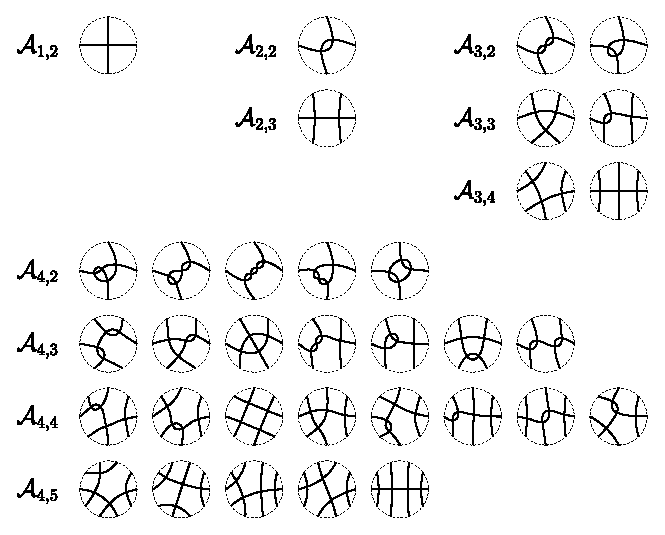
\includegraphics{c/alternating-tangles-1-4.eps}
			\caption{Альтернированные танглы до 4-х перекрестков\label{figure:tangles14}}
		\end{figure}

		\begin{figure}[ht]
			\centering
			\includegraphics{c/alternating-tangles-5.eps}
			\caption{Альтернированные танглы c 5-ю перекрестками\label{figure:tangles5}}
		\end{figure}

		\begin{landscape}
		\begin{table}[ht]
			\caption{Количество альтернированных $k$-танглов с $n$ перекрестками.\label{table:alternating-tangles-table}}
			\centering
			\begin{tabular}{|c||r|r|r|r|r|r|r|r|r|r|r|r|}
			\hline
			$k$\textbackslash $n$
			    & 1 & 2 & 3 &  4 &   5 &   6 &      7 &       8 &        9 &          10 &           11 &            12 \\
			\hline\hline
			2   & 1 & 1 & 2 &  5 &  13 &  36 &    111 &     373 &   1\,362 &      5\,378 &      22\,807 &      102\,617 \\
			3   & . & 1 & 2 &  7 &  20 &  77 &    276 &  1\,135 &   4\,823 &     21\,734 &     101\,307 &      488\,093 \\
			4   & . & . & 2 &  8 &  37 & 157 &    687 &  3\,052 &  13\,981 &     65\,797 &     317\,506 &   1\,565\,163 \\
			5   & . & . & . &  5 &  31 & 209 & 1\,128 &  5\,986 &  30\,556 &    155\,964 &     795\,918 &   4\,092\,027 \\
			6   & . & . & . &  . &  16 & 161 & 1\,294 &  8\,528 &  51\,475 &    294\,366 &  1\,637\,855 &   8\,979\,493 \\
			7   & . & . & . &  . &   . &  60 &    840 &  8\,206 &  62\,895 &    428\,254 &  2\,702\,902 &  16\,313\,106 \\
			8   & . & . & . &  . &   . &   . &    261 &  4\,702 &  52\,815 &    460\,189 &  3\,475\,551 &  23\,979\,733 \\
			9   & . & . & . &  . &   . &   . &      . &  1\,243 &  26\,753 &    341\,878 &  3\,327\,424 &  27\,625\,056 \\
			10  & . & . & . &  . &   . &   . &      . &       . &   6\,257 &    155\,593 &  2\,221\,544 &  23\,869\,621 \\
			11  & . & . & . &  . &   . &   . &      . &       . &        . &     32\,721 &     916\,595 &  14\,473\,275 \\
			12  & . & . & . &  . &   . &   . &      . &       . &        . &           . &     175\,760 &   5\,464\,661 \\
			13  & . & . & . &  . &   . &   . &      . &       . &        . &           . &            . &      963\,900 \\
			\hline
			все & 1 & 2 & 6 & 25 & 117 & 700 & 4\,597 & 33\,225 & 250\,917 & 1\,961\,874 & 15\,695\,169 & 127\,916\,745 \\
			\hline
			\end{tabular}
		\end{table}
		\end{landscape}

	\newpage
\section{Алгоритмы рисования диаграмм $k$-танглов}
	\label{section:drawing}

	Общая идея подобных алгоритмов рисования выглядит следующим образом: мы кодируем картинку конечным
	набором чисел, а затем сопоставляем каждой такой конфигурации числовое значение энергии с помощью
	некоторого выбираемого из эстетических соображений отображения. Затем с помощью какого-либо метода
	оптимизации мы находим изображение, соответствующее минимальной энергии --- это и будет результатом.

	Однако, чтобы получить картинки хорошего качества, надо использовать достаточно сложную функцию
	энергии, нахождение глобального минимума которой, вообще говоря, весьма нетривиальная задача. Еще одной
	проблемой является требование изотопности картинки изображаемой конфигурации --- со сложной
	функцией гарантировать его выполнение в глобальном минимуме практически невозможно. Поэтому мы будем
	строить изображение в две стадии --- сначала, используя максимально простую энергетическую функцию,
	получим начальное приближение, а потом, уже со сложной функцией, улучшим его методом градиентного
	спуска.

	\begin{figure}[ht]
		\centering
		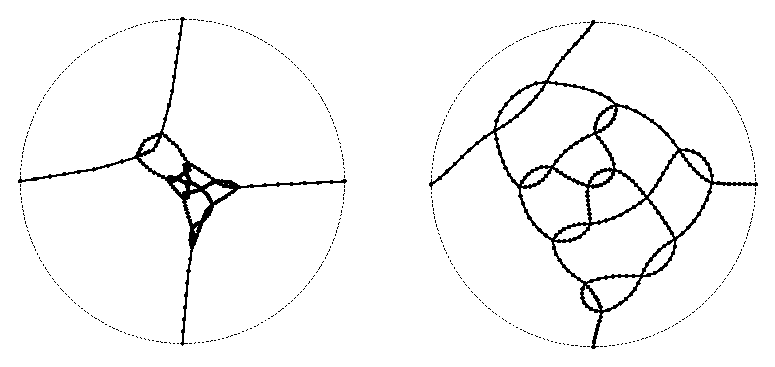
\includegraphics{c/drawing-energy.eps}
		\caption{Начальное приближение и градиентный спуск\label{figure:draw-optimization}}
	\end{figure}

	\subsection{Начальное приближение}

	На начальном этапе мы будем использовать простейшую возможную энергетическую функцию ---
	квадратичную форму
	$$
		E(x) = x \cdot Ax + b \cdot x
	$$
	Ее достоинствами являются простая физическая интерпретация как упругих взаимодействий и то, что минимум
	(если, конечно, он существует и единственен) легко найти из уравнения
	$$
		(A + A^T)x_{min} + b = 0
	$$

	Однако такой простейший подход, как выбрать в качестве переменных координаты перекрестков, а ребра представить
	упругими ``пружинками'' не приводит к желаемому результату (см.~\figureref{figure:degenerate-elastic}).
	\begin{figure}[ht]
		\centering
		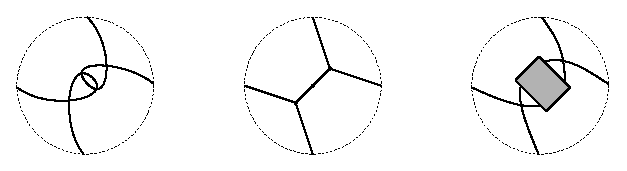
\includegraphics{c/drawing-initial-degeneration.eps}
		\caption{Диаграммы, вырождающиеся при утягивании\label{figure:degenerate-elastic}}
	\end{figure}

	Решить эту проблему можно при помощи добавления к графу дополнительных ребер-растяжек. Поместим в середину
	каждого исходного ребра тангла и каждой дуги границы-окружности дополнительный узел. Дополнительные узлы
	соединим между собой растяжками как показано на \figureref{figure:extra-elastic}. Можно представлять себе эти
	дополнительные ребра как стороны многоугольников, вписанных в грани исходного графа
	(\figureref{figure:extra-elastic}a), или же иначе --- как стяжки, попарно соединяющие соседние ребра, исходящие
	из каждой вершины тангла (\figureref{figure:extra-elastic}b).

	\begin{figure}[ht]
		\centering
		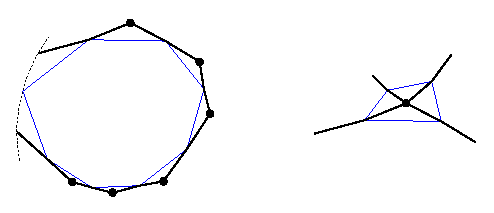
\includegraphics{c/drawing-face-crossing.eps}
		\caption{Дополнительные растяжки\label{figure:extra-elastic}}
	\end{figure}

	\begin{figure}[ht]
		\centering
		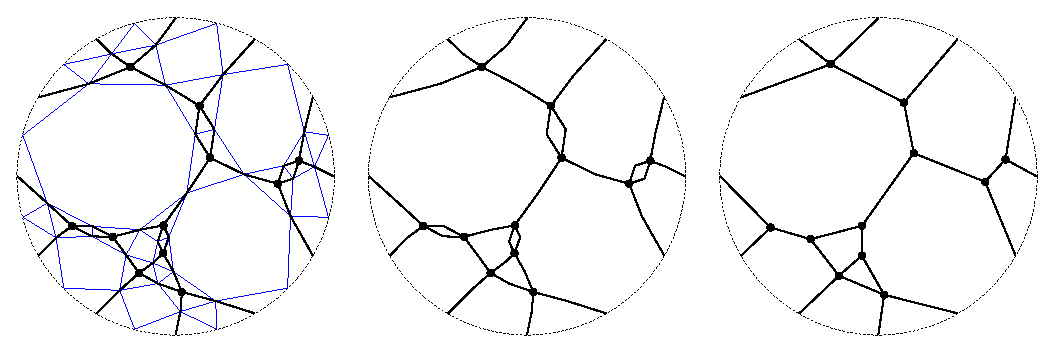
\includegraphics[scale=0.7]{c/drawing-initial-configuration-example.eps}
		\caption{Начальная конфигурация с растяжками и без\label{figure:startconfig}}
	\end{figure}

	При этом в каждой из 2-угольных граней мы получим две совпадающих растяжки. Оставим из них одну. Если у исходного
	тангла было $n$ перекрестков и $k$ концов, то полученный в результате граф содержит $n$ 4-валентных вершин
	(перекрестки исходного тангла), $k$ вершин валентности 2 (фиксированные дополнительные вершины на окружности)
	и $2n + k/2$ 5-6-валентных вершин (сколько ребер в графе тангла, 5-валентные вершины лежат на ребрах 2-угольных
	граней). Построим теперь для этого графа конфигурацию, соответствующую минимуму суммы квадратов длин ребер
	(см.~\figureref{figure:startconfig}).

	\subsection{Градиентный спуск}

	Второй стадией построения изображения, как и было сказано выше, является улучшение начальной конфигурации, полученной на
	предыдущем шаге. Для этого мы помещаем на каждом ребре начальной конфигурации еще по 1-2 промежуточных узла и запускаем
	метод градиентного спуска с новой более сложной энергетической функцией. В процессе мы должны следить за тем, чтобы за
	одну итерацию не происходило слишком больших прыжков, могущих изменить топологию текущей конфигурации, то есть ограничивать
	большие прыжки сверху.

	Основные требования к функционалу энергии для градиентного спуска:
	\begin{enumerate}
		\item
		бесконечный потенциальный барьер, препятствующий прохождению узлов через звенья;

		\item
		обращение в бесконечность при наложении ребер и стягивании в точку граней графа;

		\item
		непрерывность касательных в перекрестках;

		\item
		сходимость при увеличении числа точек на ребро;

		\item
		эстетические критерии --- хорошая различимость всех перекрестков и примерно равномерное распределение их в круге,
		длины ребер примерно равны, углы в перекрестках близки к прямым, плавное изменение кривизны
	\end{enumerate}

	Предлагаемая энергетическая функция будет линейной комбинацией четырех компонент: электростатического отталкивания элементов
	диаграммы друг от друга, электростатического отталкивания от граничной окружности, силы упругости ребер и ``изгибной''
	энергии, стремящейся спрямлять картинку в вершинах степени 2 и добиваться перпендикулярности входящих ребер в вершинах
	степени 4.

	Энергия электростатического отталкивания типа ``узел-узел'' не удовлетворяет самому важному требованию --- не обеспечивает
	потенциального барьера изменению топологии. Кроме того, рельеф потенциальной функции изобилует ямами. Энергия отталкивания
	типа ``звено-звено'' обеспечивает барьер, однако выражается довольно громоздкими формулами. Есть также проблема с вычислением
	сил взаимодействия сцепленных (инцидентных одной вершине) ребер. Наиболее подходящей кажется смешанная энергия ``звено-узел''.
	Будем считать, что заряд равномерно распределен по длине ребер тангла с единичной плотностью, но силы отталкивания сосредоточены
	в узлах, заряды которых пропорциональны полусумме длин соседних ребер. Такая схема соответствует вычислению повторного интеграла
	энергии при помощи смешанной квадратурной формулы --- одно интегрирование выполняется методом трапеций, а другое --- методом
	центральных прямоугольников.
	\begin{figure}[ht]
		\centering
		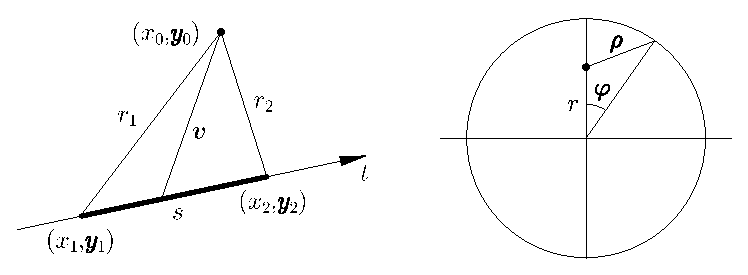
\includegraphics{c/drawing-energy-definition.eps}
		\caption{К определению электростатического потенциала взаимодействия\label{figure:electrostatic}}
	\end{figure}
	Электростатический потенциал, создаваемый заряженным отрезком (см.~\figureref{figure:electrostatic}):
	\begin{eqnarray*}
		\phi(x_0, y_0)
		= \int_0^s\frac{dt}{|\vec{v}|}
		= s\int_0^1\frac{d\tau}{\bigl([\xi_1(1-\tau)+\xi_2\tau]^2+[\eta_1(1-\tau)+\eta_2\tau]^2\bigr)^{1/2}} = {}\\
		= \ln\biggl(\frac{r_1+r_2+s}{r_1+r_2-s}\biggr)
	\end{eqnarray*}
	Здесь $\xi_{1,2}=x_0-x_{1,2}$, $\eta_{1,2}=y_0-y_{1,2}$; остальные обозначения приведены на~\figureref{figure:electrostatic}.

	Электростатический потенциал заряженной окружности единичного радиуса в ее плоскости (см.~~\figureref{figure:electrostatic}):
	$$
		\phi(r)=2\int_0^{\pi}\frac{d\phi}{\rho}=\frac{4}{1+r}\mathsf{K}\Bigl(\frac{4r}{(1+r)^2}\Bigr),
	$$
	где $\mathsf{K}()$ --- полный эллиптический интеграл 1-го рода.

	Изгибную энергию введем следующим образом. Для ломаной, заданной вершинами $p_k$, построим в каждой вершине векторы, равные
	сумме исходящих из данной вершины векторов звеньев (см.~\figureref{figure:bend-energy}). Определим изгибную энергию ломаной
	как сумму квадратов длин полученных векторов:
	$$
		E=\sum_k (x_{k-1}-2x_k+x_{k+1})^2+(y_{k-1}-2y_k+y_{k+1})^2
	$$
	Здесь $x_k$, $y_k$ --- координаты вершины $p_k$ ломаной.
	\begin{figure}[ht]
		\centering
		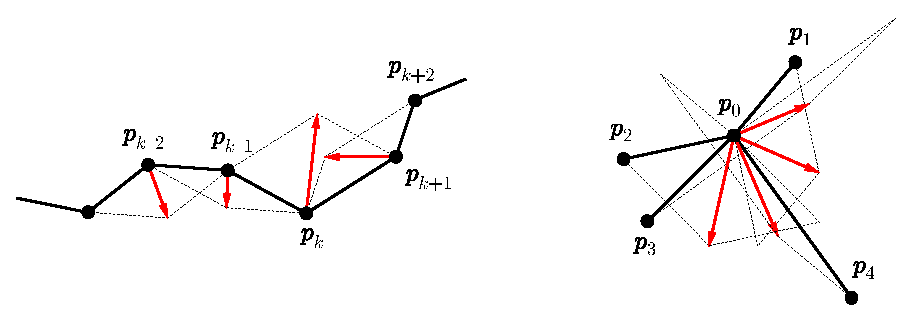
\includegraphics{c/drawing-bend-energy.eps}
		\caption{К определению изгибной энергии\label{figure:bend-energy}}
	\end{figure}
	Такая изгибная энергия равна нулю только для равнозвенной прямолинейной ломаной. Компоненты градиента изгибной энергии представляют
	собой разности 4-го порядка последовательности координат вершин:
	\begin{eqnarray*}
		\frac{\partial E}{\partial x_k} = x_{k-2} - 4x_{k-1} + 6x_k - 4x_{k+1} + x_{k+2} \\ [10pt]
		\frac{\partial E}{\partial y_k} = y_{k-2} - 4y_{k-1} + 6y_k - 4y_{k+1} + y_{k+2}
	\end{eqnarray*}

	Аналогичную функцию можно использовать для того чтобы выполнить еще одно требование к ``хорошо нарисованной'' проекции --- дуги в
	перекрестках должны пересекаться под приблизительно прямым углом. Обозначим узлы, соседние с данным перекрестком, в порядке против
	часовой стрелки, $p_1$, $p_2$, $p_3$ и $p_4$ (см.~\figureref{figure:bend-energy}) и введем соответствующие векторы, исходящие из
	перекрестка: $(x_1 - x_0, y_1 - y_0)$ и т.д. Мерой перпендикулярности двух последовательных векторов может служить вектор --- сумма
	одного из них с перпендикулярной копией второго. Энергию перекрестка определим как сумму квадратов длин таких векторов:
	\begin{eqnarray*}
		E = (x_2-x_0+y_1-y_0)^2 + (y_2-y_0-x_1+x_0)^2 + (x_3-x_0+y_2-y_0)^2 + \\
		+ (y_3-y_0-x_2+x_0)^2 + (x_4-x_0+y_3-y_0)^2 + (y_4-y_0-x_3+x_0)^2 + \\
		+ (x_1-x_0+y_4-y_0)^2 + (y_1-y_0-x_4+x_0)^2
	\end{eqnarray*}
	Это выражение обращается в ноль лишь когда все четыре вектора равны по величине, и все углы прямые.

	\newpage
\section{Заключение}
	Все известные алгоритмы перечисления объектов теории узлов работают похожим образом: сначала каким-то образом генерируются
	все ``интересные'' диаграммы исследуемых объектов, затем с помощью определенных инвариантов и хеш-таблиц из полученного
	множества диаграмм удаляются повторы, соответствующие одному и тому же объекту. Например, в процессе перечисления альтернированных
	зацеплений в \cite{Rankin2002_1, Rankin2002_2, Rankin2002_3} для генерации диаграмм использовались локальные преобразования,
	как на \figureref{figure:surgeries}, а удаление дубликатов производилось с помощью введенного авторами полного инварианта
	``Master Array''.
	\begin{figure}[ht]
		\centering
		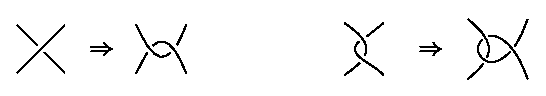
\includegraphics{c/surgeries.eps}
		\caption{Локальные преобразования\label{figure:surgeries}}
	\end{figure}

	Очевидным недостатком такой схемы являются необходимость поддерживать хеш-таблицу очень больших размеров и выполнять поиск
	по ней. Также часто возникает проблема с тем, что доля заведомо бесполезной работы с увеличением размера объектов возрастает
	экспоненциально, так как экспоненциально растет доля повторяющихся диаграмм. Предложенный в данной работе тип алгоритмов
	свободен от подобного рода проблем. Перебор проекций в Главе~\ref{section:projections} вообще не требует хранения уже
	полученных им объектов, а алогоритм генерации альтернированных $k$-танглов из Главы~\ref{section:alternating} не требует
	поиска и хранит только малую часть сгенерированного. Доля лишней работы растет не более чем линейно с ростом максимального
	числа концов.

	Еще одним достоинством предложенной схемы является широкая возможность ее обобщения. В качестве примера, легко понять как
	приспособить ее для генерации полимино, или диаграмм альтернированных зацеплений, или, возможно, самих альтернированных
	зацеплений.

	Вероятным следующим шагом могло бы явится обобщение алгоритма на неальтернированные $k$-танглы, впрочем в этом случае такое
	свойство, как отсутствие поисковых запросов по уже сгенерированным объектам, скорее всего не удастся сохранить.

	Реализации на языке C++ приведенных алгоритмов можно найти по адресу \uline{http://code.google.com/p/tanglenum/}.

	\newpage
\renewcommand{\bibname}{Список литературы}
\begin{thebibliography}{99}
	\addcontentsline{toc}{section}{\bibname}

	\bibitem{Conway1970}
	Conway J. An enumeration of knots and links, and some of their algebraic
	properties. Computational Problems in Abstract Algebra (John Leech, ed.), Pergamon Press, Oxford
	and New York, 1969, 329-358.

	\bibitem{Cromwell2004}
	Cromwell P. Knots and links. Cambridge: Cambridje university press. 2004. 350~p.

	\bibitem{KanenobuSaitoSatoh2003}
	Kanenobu T., Saito H., and Satoh S. Tangles with up to seven crossings.
	Interdisciplinary Information Sciences, Vol. 9, No. 1, pp. 127-140 (2003).

	\bibitem{KauffmanLambropoulou2004}
	Kauffman L., Lambropoulou S. On the classification of rational tangles.
	Advances in Applied Mathematics Volume 33, Issue 2, August 2004, Pages 199-237.
	e-print:~\texttt{arXiv:math/0311499v2}

	\bibitem{Justin1999_1}
	Zinn-Justin P. Matrix Integrals and the Counting of Tangles and Links.
	e-print:~\texttt{arXiv:math-ph/9904019v2}

	\bibitem{Justin1999_2}
	Zinn-Justin P. Some Matrix Integrals related to Knots and Links
	e-print:~\texttt{arXiv:math-ph/9910010v1}

	\bibitem{JustinZuber2000}
	Zinn-Justin P., Zuber J. On the Counting of Colored Tangles.
	e-print:~\texttt{arXiv:math-ph/0002020v2}

	\bibitem{Justin2001}
	Zinn-Justin P. The General O(n) Quartic Matrix Model and its application to Counting Tangles and Links.
	e-print:~\texttt{arXiv:math-ph/0106005v1}

	\bibitem{JacobsenJustin2002}
	Jacobsen J.L., Zinn-Justin P. The combinatorics of alternating tangles:
	from theory to computerized enumeration. e-print:~\texttt{arXiv:math-ph/0111011v1}

	\bibitem{JustinZuber2003}
	Zinn-Justin P., Zuber J. Matrix integrals and the generation and counting
	of virtual tangles and links. J.Knot Theor.Ramifications 13 (2004) 325-356.
	e-print:~\texttt{arXiv:math-ph/0303049}

	\bibitem{Kauffman1999}
	Kauffman L. Virtual knot theory. European Journal of Combinatorics. 1999.
	20. P.663--690.  e-print:~\texttt{arXiv:math/9811028v3}

	\bibitem{Kuperberg2003}
	Kuperberg G. What is a virtual link? Algebr. Geom. Topol. 3 (2003) 587--591.
	e-print:~\texttt{arXiv:math/0208039v2}

	\bibitem{Tait1900}
	Tait, P.G. On Knots I, II, III. Scientific Papers, Vol. 1. London: Cambridge University Press, pp. 273--347, 1900.

	\bibitem{MenascoThistlethwaite1991}
	Menasco, W. and Thistlethwaite, M. The Tait Flyping Conjecture. Bull. Amer. Math. Soc. 25, 403--412, 1991. 

	\bibitem{MenascoThistlethwaite1993}
	Menasco, W. and Thistlethwaite, M. The Classification of Alternating Links. Ann. Math. 138, 113--171, 1993.

	\bibitem{SundbergThistlethwaite1998}
	Sundberg, C. and Thistlethwaite, M. The Rate of Growth of the Number of Prime Alternating Links and Tangles.
	Pacific Journal of Mathematics, Vol. 182, No. 2, pp. 329--358, 1998.

	\bibitem{Rankin2002_1}
	Rankin S., Schermann J., Smith O. Enumerating the prime alternating knots, Part	I,
	Journal of Knot Theory and Its Ramifications, Vol. 13, No. 1 (2004) 57-100
	e-print:~\texttt{arXiv:math/0211346}

	\bibitem{Rankin2002_2}
	Rankin S., Schermann J., Smith O. Enumerating the prime alternating knots, Part II,
	Journal of Knot Theory and Its Ramifications, Vol. 13, No. 1 (2004) 101-149
	e-print:~\texttt{arXiv:math/0211348}

	\bibitem{Rankin2002_3}
	Rankin S., Smith O. Enumerating the Prime Alternating Links
	Journal of Knot Theory and Its Ramifications, Vol. 13, No. 1 (2004) 151-173
	e-print:~\texttt{arXiv:math/0211451}

\end{thebibliography}

\end{document}
